\documentclass[11pt]{article}
\usepackage[utf8]{inputenc}
%\geometry{showframe}% for debugging purposes -- displays the margins

\newcommand{\E}{\mbox{E}}
\newcommand{\MSE}{\mbox{MSE}}
\newcommand{\var}{\mbox{var}}
\newcommand{\by}{\textbf{y}}

%% ys
\usepackage[shortlabels]{enumitem}
\usepackage{geometry}
\usepackage{bm}
\usepackage{amssymb}
\usepackage{algorithm}
\usepackage{algpseudocode}
\usepackage{xcolor}
\usepackage{listings}
\geometry{a4paper,scale=0.75}
\newcommand{\jie}{$\star$ }
\newcommand{\bx}{\bm{x}}
\newcommand{\iid}{\overset{\text{iid}}{\sim}}
\newcommand{\half}{\frac{1}{2}}
\newcommand{\ynote}[1]{\color{red} #1 \color{black}}
%% ys

\usepackage{amsmath}
%\usepackage[garamond]{mathdesign}
\usepackage{url}

% Set up the images/graphics package
\usepackage{graphicx}
\setkeys{Gin}{width=\linewidth,totalheight=\textheight,keepaspectratio}
\graphicspath{{graphics/}}

\title{Exercises 4 $\cdot$ SDS 383D \\ Exercises 4: Intro to Hierarchical Models}
\author{Yunshan Duan }
\date{}  % if the \date{} command is left out, the current date will be used

% The following package makes prettier tables.  We're all about the bling!
\usepackage{booktabs}

% The units package provides nice, non-stacked fractions and better spacing
% for units.
\usepackage{units}

% The fancyvrb package lets us customize the formatting of verbatim
% environments.  We use a slightly smaller font.
\usepackage{fancyvrb}
\fvset{fontsize=\normalsize}

% Small sections of multiple columns
\usepackage{multicol}

% Provides paragraphs of dummy text
\usepackage{lipsum}

% These commands are used to pretty-print LaTeX commands
\newcommand{\doccmd}[1]{\texttt{\textbackslash#1}}% command name -- adds backslash automatically
\newcommand{\docopt}[1]{\ensuremath{\langle}\textrm{\textit{#1}}\ensuremath{\rangle}}% optional command argument
\newcommand{\docarg}[1]{\textrm{\textit{#1}}}% (required) command argument
\newenvironment{docspec}{\begin{quote}\noindent}{\end{quote}}% command specification environment
\newcommand{\docenv}[1]{\textsf{#1}}% environment name
\newcommand{\docpkg}[1]{\texttt{#1}}% package name
\newcommand{\doccls}[1]{\texttt{#1}}% document class name
\newcommand{\docclsopt}[1]{\texttt{#1}}% document class option name

\newcommand{\N}{\mbox{N}}
\newcommand{\thetahat}{\hat{\theta}}
\newcommand{\sigmahat}{\hat{\sigma}}
\newcommand{\betahat}{\hat{\beta}}


\begin{document}

\maketitle% this prints the handout title, author, and date


\section{Math tests}

The data set in ``mathtest.csv'' shows the scores on a standardized math test from a sample of 10th-grade students at $P=100$ different U.S.~urban high schools, all having enrollment of at least 400 10th-grade students.  (A lot of educational research involves ``survey tests'' of this sort, with tests administered to all students being the rare exception.)

Let $\theta_i$ be the underlying mean test score for school $i$, and let $y_{ij}$ be the score for the $j$th student in school $i$.  Our main parameter of interest is $\theta$, the vector of school-level means.  We'll assume that each student's test score is normally distributed around the corresponding school-level mean: $y_{ij} \sim \mbox{N}(\theta_i, \sigma^2)$ for $i=1, \ldots, P$ and $j = 1, \ldots, N_i$.  

\begin{enumerate}[(A)]
\item Show (somewhat trivially) that the maximum likelihood estimate for $\theta$ is just the vector of sample means: $\hat{\theta}_{\mathrm{MLE}} = (\bar{y}_1, \ldots, \bar{y}_P)$.  

\bigskip
\jie
The likelihood is
$$p(y \mid \theta) \propto \prod_{i=1}^P \prod_{j=1}^{N_i} \exp\{-\frac{1}{2} (y_{ij} - \theta_i)^2\}.$$
Then,
$$\frac{\partial}{\partial \theta_i} \log L = \sum_{j=1}^{N_i} (y_{ij} - \theta_i).$$
Therefore, the MLE 
$$\hat{\theta}_i = \frac{1}{N_i} \sum_{j=1}^{N_i} y_{ij} = \bar{y}_i,$$
i.e. $\hat{\theta}_{\mathrm{MLE}} = (\bar{y}_1, \ldots, \bar{y}_P)$.
\bigskip

\item Make a plot that illustrates the following fact: extreme school-level averages $\bar{y}_i$ (both high and low) tend to be at schools where fewer students were sampled.  Explain briefly why this would be.
\bigskip
\jie
Figure \ref{fig:bary_n} shows that extreme school-level averages have fewer students. The reason for this might be those school with high averages are harder to get into and schools with extreme low averages cannot recruit as much student as the ones are better.
\begin{figure}[h]
    \centering
    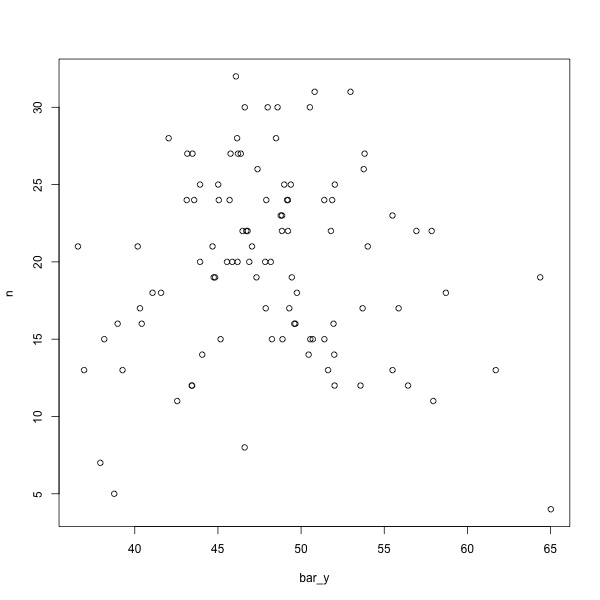
\includegraphics[width=0.6\textwidth]{Ex4/figures/bary_n.jpeg}
    \caption{Average score of each school v.s. number of students.}
    \label{fig:bary_n}
\end{figure}

\item Fit the following two-level hierarchical model to these data via Gibbs sampling:
\begin{eqnarray*}
(y_{ij} \mid \theta_i, \sigma^2) &\sim& \mbox{N}(\theta_i, \sigma^2) \\
(\theta_i \mid \tau^2, \sigma^2) &\sim& \mbox{N}(\mu, \tau^2 \sigma^2)
\end{eqnarray*}

As a starting point, use a flat prior on $\mu$, Jeffreys' prior on $\sigma^2$, and an inverse-gamma(1/2, 1/2) prior on $\tau^2$.  Your Gibbs sampler should cycle between the complete conditional posterior distributions for each of these parameters in turn, as well as $\theta$ (the vector of means).  While you could update each $\theta_i$ individually, I encourage you to think about it as a vector whose conditional distribution is multivariate normal, and whose covariance matrix happens to be diagonal.  This view will generalize more readily to future problems.  

\item Express the conditional posterior mean for $\theta_i$ in the following form:
$$
E(\theta_i \mid y, \tau^2, \sigma^2, \mu) = \kappa_i \mu + (1-\kappa_i) \bar{y}_i \, ,
$$
i.e. a convex combination of prior mean and data mean.  Here $\kappa_i$ is a \textit{shrinkage coefficient} whose form you should express in terms of the model hyperparameters.  In the extreme case where $\kappa_i$ is 1, then the data ($\bar{y}_i$) are essentially ignored, and the posterior mean is ``shrunk'' all the way back to the prior mean.  In the other extreme where $\kappa_i$ is 0, the prior mean is ignored, and the posterior mean is entirely ``un-shrunk'' compared to the MLE for $\theta_i$.  

For each draw of your MCMC, calculate $\kappa_i$ for each school, and save the posterior draws.  Average these MCMC samples to calculate $\bar{\kappa}_i$, the posterior mean of this shrinkage coefficient.   Plot $\bar{\kappa}_i$ for each school as a function of that school's sample size, and comment on what you see.  

\item Observe that an equivalent way to write your model involves the following decomposition:  
$$
y_{ij} = \mu + \delta_i + e_{ij}
$$
where $\delta_i \sim N(0, \tau^2 \sigma^2)$ and $e_{ij} \sim N(0, \sigma^2)$.  (In the paper by Gelman that I've asked you to read, he writes it this way, where the school-level ``offsets'' are centered at zero, although he doesn't scale these offsets by $\sigma$ the way I prefer to do.)  To translate between the two parameterizations, just observe that in the previous version, $\theta_i = \mu + \delta_i$.  

Conditional on the ``grand mean'' $\mu$, but \emph{marginally} over both $\delta_i$ and $e_{ij}$, compute the following two covariances:

\begin{compactitem}
\item $\mbox{cov}(y_{i,j}, y_{i,k})$, $j \neq k$
\item $\mbox{cov}(y_{i,j}, y_{i', k})$, $i \neq i'$ and $j \neq k$
\end{compactitem}

Does this make sense to you?  Why or why not?  

\item Does the assumption that $\sigma^2$ is common to all schools look justified in light of the data?  

\end{enumerate}


\section{Blood pressure}

The data set in ``bloodpressure.csv'' contains data on repeated blood pressure measurements on 20 different subjects, ten of whom received a control medication (treatment=1) and ten of whom received an experimental medication (treatment = 2).  Patients were randomized to receive the two treatments.  The columns are the data of measurement, a numerical ID for the subject, the blood pressure measurement (systolic), and which treatment the patient received.

\begin{enumerate}[(A)]

\item Is the experimental medication effective at reducing blood pressure?  Do the naive thing and perform a t-test for a difference of means, pooling all the data from treatment 1 into group 1, and all the data from treatment 2 into group 2.  What does this t-test say about the difference between these two group means, and the standard error for the difference?  Why is the t-test (badly) wrong?

\item Now do something better, but still less than ideal.  Calculate $\bar{y}_i$, the mean blood pressure measurement for each patient.  Now treat each person-level mean as if it were just a single data point, and conduct a different t-test for mean blood pressure between treatment 1 and treatment 2.  (If you're doing this correctly, you should have only ten "observations" in each group, where each observation is actually a person-level mean.) What does this t-test say about the difference between these two group means, and the standard error for the difference?  Why is the standard error so much bigger, and why is this appropriate?  Even so, why is this approach (subtly) wrong?  

\item Now fit a two-level hierarchical model to this data, of the following form:
\begin{eqnarray*}
(y_{ij} \mid \theta_i, \sigma^2) &\sim& \mbox{N}(\theta_i, \sigma^2) \\
(\theta_i \mid \tau^2, \sigma^2) &\sim& \mbox{N}(\mu + \beta x_i, \tau^2 \sigma^2)
\end{eqnarray*}
where $y_{ij}$ is blood pressure measurement $j$ on person $i$, and $x_i$ is a dummy (0/1) variable indicating whether a patient received treatment 2, the experimental medication.   Apply what you learned on the previous problem about sampling, hyperparameters, etc, but account for the extra wrinkle here, i.e. the presence of the $\beta x_i$ term that shifts the mean between the treatment and control groups.  

Write our your model's complete conditional distributions, and fit it.  Make a histogram of the posterior distribution for $\beta$, which represents the treatment effect here.  In particular, what are the posterior mean and standard deviation of $\beta$?  How do these compare to the estimates and standard errors from the approaches in (A) and (B)?  

\item Your two-level model assumes that, conditional on $\theta_i$, the $y_{ij}$ are independent.  Written concisely: $(y_{ij} \perp y_{ik} \mid \theta_i)$ for $j \neq k$. 

There are many ways this assumption could break down.  So check!  Does this assumption look (approximately) sensible in light of the data?  Provide evidence one way or another.  

\end{enumerate}


%
%\subsection{Price elasticity of demand}
%
%The data in ``cheese.csv'' are about sales volume, price, and advertisting display activity for packages of Borden sliced ``cheese.'' The data are taken from Rossi, Allenby, and McCulloch's textbook on \textit{Bayesian Statistics and Marketing.} For each of 88 stores (store) in different US cities, we have repeated observations of the weekly sales volume (vol, in terms of packages sold), unit price (price), and whether the product was advertised with an in-store display during that week (disp = 1 for display).
%
%Your goal is to estimate, on a store-by-store basis, the effect of display ads on the demand curve for cheese.  A standard form of a demand curve in economics is of the form $Q = \alpha P^\beta$, where $Q$ is quantity demanded (i.e.~sales volume), $P$ is price, and $\alpha$ and $\beta$ are parameters to be estimated.  You'll notice that this is linear on a log-log scale,
%$$
%\log Q = \log \alpha + \beta \log P \,
%$$
%which you should feel free to assume here.  Economists would refer to $\beta$ as the price elasticity of demand (PED).  Notice that on a log-log scale, the errors enter multiplicatively.
%
%There are several things for you to consider in analyzing this data set.
%\begin{compactenum}
%\item The demand curve might shift (different $\alpha$) and also change shape (different $\beta$) depending on whether there is a display ad or not in the store.
%\item Different stores will have very different typical volumes, and your model should account for this.
%\item Do different stores have different PEDs?  If so, do you really want to estimate a separate, unrelated $\beta$ for each store?
%\item If there is an effect on the demand curve due to showing a display ad, does this effect differ store by store, or does it look relatively stable across stores?
%\item Once you build the best model you can using the log-log specification, do see you any evidence of major model mis-fit?
%\end{compactenum}
%Propose an appropriate hierarchical model that allows you to address these issues, and use Gibbs sampling to fit your model.
%
%
\end{document}

